\documentclass[]{article}
\usepackage[T1]{fontenc}
\usepackage{lmodern}
\usepackage{amssymb,amsmath, graphicx}
\usepackage{ifxetex, ifluatex, floatflt}
\usepackage{fixltx2e} % provides \textsubscript
% use upquote if available, for straight quotes in verbatim environments
\IfFileExists{upquote.sty}{\usepackage{upquote}}{}
\ifnum 0\ifxetex 1\fi\ifluatex 1\fi=0 % if pdftex
\usepackage[utf8]{inputenc}
\else % if luatex or xelatex
\ifxetex
\usepackage{mathspec}
\usepackage{xltxtra,xunicode}
\else
\usepackage{fontspec}
\fi
\defaultfontfeatures{Mapping=tex-text,Scale=MatchLowercase}
\newcommand{\euro}{€}
\fi
% use microtype if available
\IfFileExists{microtype.sty}{\usepackage{microtype}}{}
\ifxetex
  \usepackage[setpagesize=false, % page size defined by xetex
              unicode=false, % unicode breaks when used with xetex
              xetex]{hyperref}
\else
  \usepackage[unicode=true]{hyperref}
\fi
\hypersetup{breaklinks=true,
  bookmarks=true,
  pdfauthor={},
  pdftitle={},
  colorlinks=true,
  citecolor=blue,
  urlcolor=blue,
  linkcolor=magenta,
  pdfborder={0 0 0}}
\urlstyle{same}  % don't use monospace font for urls
\setlength{\parindent}{0pt}
\setlength{\parskip}{6pt plus 2pt minus 1pt}
\setlength{\emergencystretch}{3em}  % prevent overfull lines
\setcounter{secnumdepth}{0}

\title{nprstuff}
\date{\today}
\author{Tanim Islam}

\begin{document}
\maketitle

I like NPR, so I made some scripts to download my favorite programs from NPR. For now, I have something that downloads \href{http://www.npr.org/programs/fresh-air/}{Fresh Air},
\href{http://www.npr.org/programs/wait-wait-dont-tell-me/}{Wait Wait..Don't Tell Me}, and \href{http://www.thisamericanlife.org/}{This American Life}. This package can probably, straightforwardly be extended to other NPR and PRI programs.

Although this project started off as a way to download these three programs, I have expanded it to include a grab bag of altogether different types of functionalities. What remains the same? This distribution consists mainly of executable python scripts.

I organize this document into the following sections: Core Functionality, New Functionality, Graphics Functionality (in folders {\verb|gui|} and {\verb|gui2|}), and a small section called Oldstuff.

This document was converted from a \LaTeX source using \href{http://pandoc.org/index.html}{Pandoc}, via
\begin{verbatim}
pandoc -s README.tex -o README.rst
\end{verbatim}

\section{Core Functionality}\label{sec:core_functionality}
This consists of functionality to grab episodes from \href{http://www.npr.org/programs/fresh-air/}{Fresh Air},  \href{http://www.npr.org/programs/wait-wait-dont-tell-me/}{Wait Wait..Don't Tell Me}, and \href{http://www.thisamericanlife.org/}{This American Life}. These consist of the following pieces of python code:
\begin{itemize}
  \item {\verb|npr_utils.py|} contains common utilities to get the proper metadata for NPR programs, to name these media files in the proper date format, and to get the full paths to the \href{https://libav.org}{LibAV/FFMPEG} and \href{https://handbrake.fr/}{HandBrakeCLI} tools to create the NPR programs in m4a and mp3 formats (among other functionalities).
  
  \item These four files handle NPR Fresh Air downloads: {\verb|freshair.py|}, {\verb|freshair_crontab.py|}, {\verb|freshair_fix_crontab.py|}, and {\verb|freshair_by_year.py|}.
  \begin{itemize}
    \item {\verb|freshair.py|} is the main executable that downloads NPR Fresh Air episodes, converts them to m4a format, and then applies correct metadata. The help screen for this command line tool is here,
    \begin{verbatim}
Usage: freshair.py [options]

Options:
  -h, --help         show this help message and exit
  --dirname=DIRNAME  Name of the directory to store the file. Default is
                     /mnt/media/freshair.
  --date=DATE        The date, in the form of "January 1, 2014." The default
                     is today's date, November 14, 2015.
  --debug            If chosen, run freshair.py in debug mode. Useful for
                     debugging :)
\end{verbatim}
    
    \item {\verb|freshair_crontab.py|} downloads an NPR Fresh Air episode on a given weekday. It should be called by a cron job that should be run every weekday.
    
    \item {\verb|freshair_fix_crontab.py|} tries to re-download NPR Fresh Air episodes that may be incomplete -- defined as shorter than 30 minutes -- and which are 90 days or older. This executable searches through the library of all NPR Fresh Air episodes, and tries to re-download older, possibly incomplete episodes.
    
    \item {\verb|freshair_by_year.py|} downloads all the NPR Fresh Air episodes in a given year.
  \end{itemize}
  
  \item These four files handle NPR Wait Wait downloads: {\verb|waitwait.py|}, {\verb|waitwait_realmedia.py|}, {\verb|waitwait_crontab.py|}, and {\verb|waitwait_by_year.py|}.
  \begin{itemize}
   \item {\verb|freshair.py|} is the main executable that downloads NPR Wait Wait episodes, converts them to m4a format, and then applies correct metadata. {\verb|waitwait_realmedia.py|} is a python module that allows one to download NPR Wait Wait episodes older than 2004, which are in \href{https://en.wikipedia.org/wiki/RealMedia}{RealMedia} format. The help screen for this command line tool is here,
   \begin{verbatim}
Usage: waitwait.py [options]

Options:
  -h, --help         show this help message and exit
  --dirname=DIRNAME  Name of the directory to store the file. Default is
                     /mnt/media/waitwait.
  --date=DATE        The date, in the form of "January 1, 2014." The default
                     is last Saturday, November 14, 2015.
  --debugonly        If chosen, download the NPR XML data sheet for this Wait
                     Wait episode.
\end{verbatim}
   
   \item {\verb|waitwait_crontab.py|} downloads an NPR Wait Wait episode on a given Saturday. It should be called by a cron job that should be run every Saturday.
   
   \item {\verb|waitwait_by_year.py|} downloads all the NPR Wait Wait episodes in a given year.
  \end{itemize}

  \item {\verb|thisamericanlife.py|} \textit{manually} downloads a given episode number of This American Life. This executable uses a custom online archive for older This American Life episodes that are described \href{http://www.dirtygreek.org/t/download-this-american-life-episodes}{here}. The help screen for this command line tool is here,
  \begin{verbatim}
Usage: thisamericanlife.py [options]

Options:
  -h, --help            show this help message and exit
  --episode=EPISODE     Episode number of This American Life to download.
                        Default is 150.
  --directory=DIRECTORY
                        Directory into which to download This American Life
                        episodes. Default is /mnt/media/thisamericanlife.
  --extra=EXTRASTUFF    If defined, some extra stuff in the URL to get a This
                        American Life episode.
\end{verbatim}
\end{itemize}

\section{New Functionality}\label{sec:new_functionality}
This consists of newer functionality that does not download NPR episodes, nor can one straightforwardly modify them to download NPR episodes. These consist of the following pieces of python code.
\begin{itemize}
 \item {\verb|autoCropImage.py|} automatically crops image (png, jpeg, tiff, etc.) files to remove whitespace. The default whitespace color is {\verb|white|}. The help screen for this command line tool is here,
 \begin{verbatim}
Usage: autoCropImage.py [options]

Options:
  -h, --help       show this help message and exit
  --input=INPUT    Name of the input file.
  --output=OUTPUT  Name of the output file. Optional.
  --color=COLOR    Name of the color over which to autocrop. Default is white.
\end{verbatim}
 
 \item {\verb|convertImage.py|} uses the \href{https://cloudconvert.com/apiconsole}{CloudConvert REST API} to \textit{smoothly and without pain points} convert and resize SVG images to PNG images of the same base name. The help screen for this command line tool is here,
 \begin{verbatim}
Usage: convertImage.py [options]

Options:
  -h, --help           show this help message and exit
  --filename=FILENAME  Name of the input SVG file.
  --width=WIDTH        If defined, new width of the file. Optional
\end{verbatim}
 
 \item {\verb|changedates.py|} changes the creation date of JPG and MOV files, that my Canon digital camera creates, by up and down one year. I created this tool because my Canon digital camera does not set the right year on the creation date for image files it creates. This caused problems when I uploaded those images to \href{https://picasaweb.google.com/home}{Google Picasa} or \href{https://plus.google.com/}{Google+}. The help screen for this command line tool is here,
 \begin{verbatim}
Usage: changedates.py [options]

Options:
  -h, --help         show this help message and exit
  --dirname=DIRNAME  Name of the directory to look for jpeg files.
  --movs             If chosen, process MOV files instead.
  --minus            If chosen, subtract a year from the files.
\end{verbatim}
 
 \item {\verb|music_to_m4a.py|} can convert a single file from mp3/ogg/flac format to m4a format while preserving music file metadata, and can optionally set the total number of album tracks and the album cover if the music files is in an album. It can also rename an m4a music file into the format ``\textit{artist name} - \textit{song name}.m4a.'' The help screen for this command line tool is here,
 \begin{verbatim}
Usage: music_to_m4a.py [options]

Options:
  -h, --help            show this help message and exit
  --inputfile=INPUTFILE
                        Name of the input audio file to convert.
  --outfile=OUTFILE     Optional name of the output file.
  --tottracks=TOTTRACKS
                        Optional total number of tracks in album of which song
                        is a part.
  --albumloc=ALBUMLOC   Optional path to location of the album cover image
                        file. Must be in JPEG or PNG.
  --quiet               If chosen, then verbosely print output of processing.
  --rename              If chosen, simply rename the m4a file to the form
                        <artist>.<song title>.m4a
\end{verbatim}
 
 \item {\verb|download_surahs.py|} downloads recorded surahs (\href{http://quranicaudio.com/quran/109}{Abdur-Rashid Sufi}) to a directory of your choice. The help screen for this command line tool is here,
 \begin{verbatim}
Usage: download_surahs.py [options]

Options:
  -h, --help       show this help message and exit
  --outdir=OUTDIR  Directory to put this data into. Default is
                   /mnt/software/sources/pythonics/nprstuff.
\end{verbatim}
\end{itemize}

\section{Graphics Functionality}\label{sec:graphics_functionality}
This section describes the two graphical tools I have developed:
{\verb|gui|} matches a small subset of functionality that the
\href{https://www.readability.com}{Readability} tool handles
excellently; {\verb|gui2|} is a
\href{https://www.riverbankcomputing.com/software/pyqt/download}{PyQt4}
GUI front-end to the \href{https://www.readability.com}{Readability}
API.

\subsection{GUI: Media Website Text Formatter} \label{subsec:gui}
This GUI can read from the following media websites:
\href{http://www.lightspeedmagazine.com/}{Lightspeed Magazine},
\href{https://medium.com/}{Medium},
\href{http://www.newyorker.com/}{The New Yorker},
\href{http://www.nytimes.com/?WT.z_jog=1}{The New York Times}, and the
\href{http://www.vqronline.org/}{Virginia Quarterly Review}. Here is a
screenshot!
\begin{figure}[!ht]
  \parbox[!ht]{0.65\linewidth}{%
    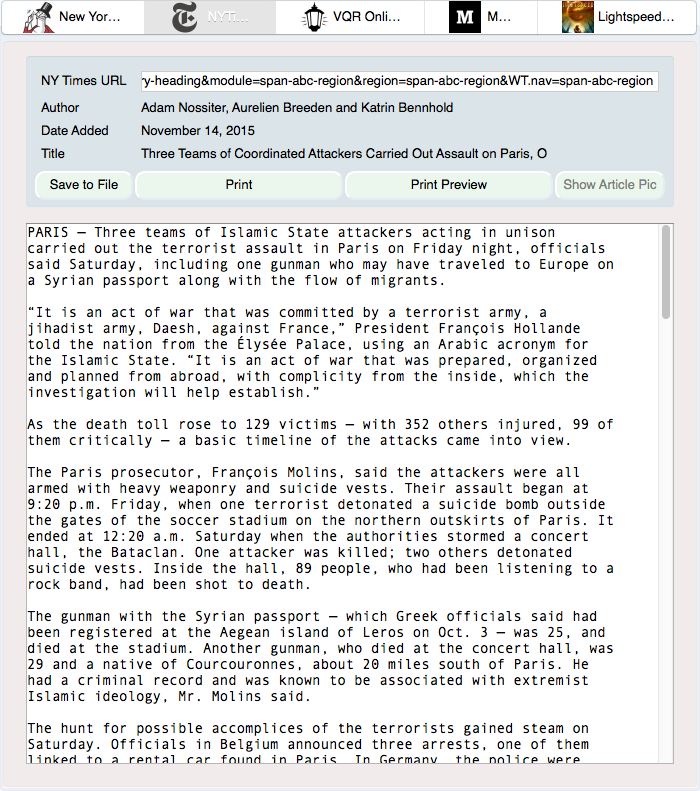
\includegraphics[width=\linewidth]{images/gui_screenshot.png}
  } \hfill
  \parbox[!ht]{0.34\linewidth}{%
    \caption{A screenshot of the GUI reader, converting the URL for
      the \href{http://www.nytimes.com}{The New York Times} into
      text. Note the separate icons above for the five media websites
      from which this GUI can read.} \label{fig:gui_screenshot}}
\end{figure}
The screenshots of the save file dialog and the print preview dialog
are shown Fig.~\ref{fig:gui_screenshot_save} and
Fig.~\ref{fig:gui_screenshot_printpreview}, respectively.
\begin{figure}[!ht]
  \parbox[!ht]{0.4\linewidth}{%
    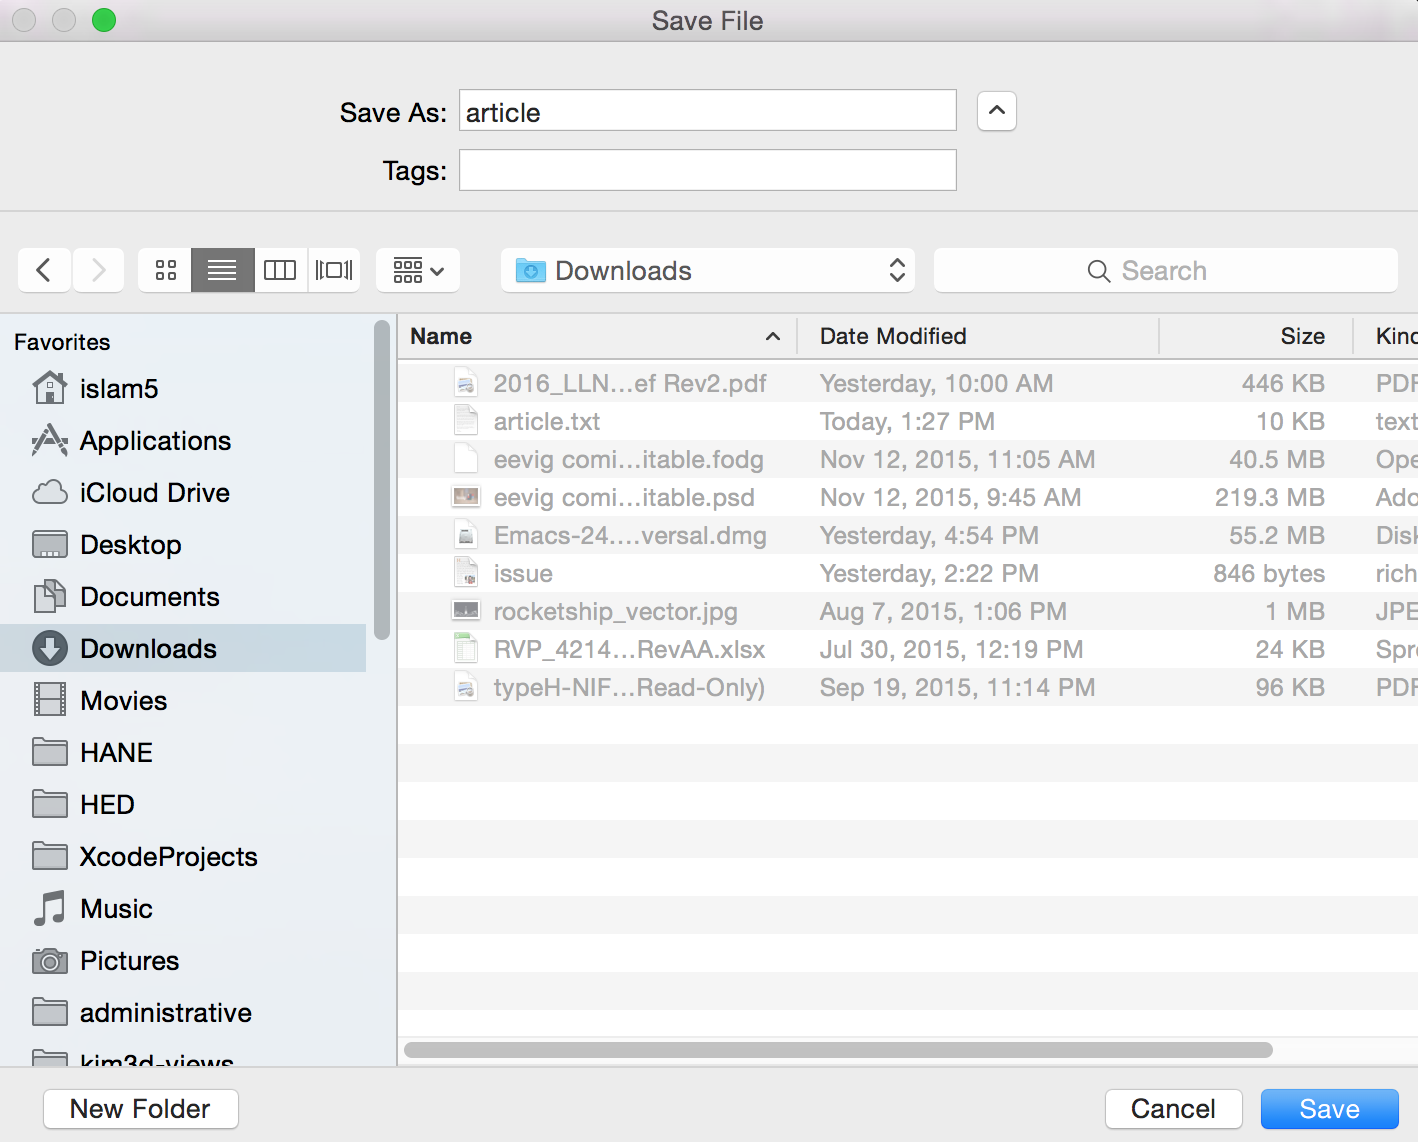
\includegraphics[width=\linewidth]{images/gui_screenshot_save.png}
    \caption{The GUI screenshot of the save
      dialog.} \label{fig:gui_screenshot_save}} \hfill
  \parbox[!ht]{0.5\linewidth}{%
    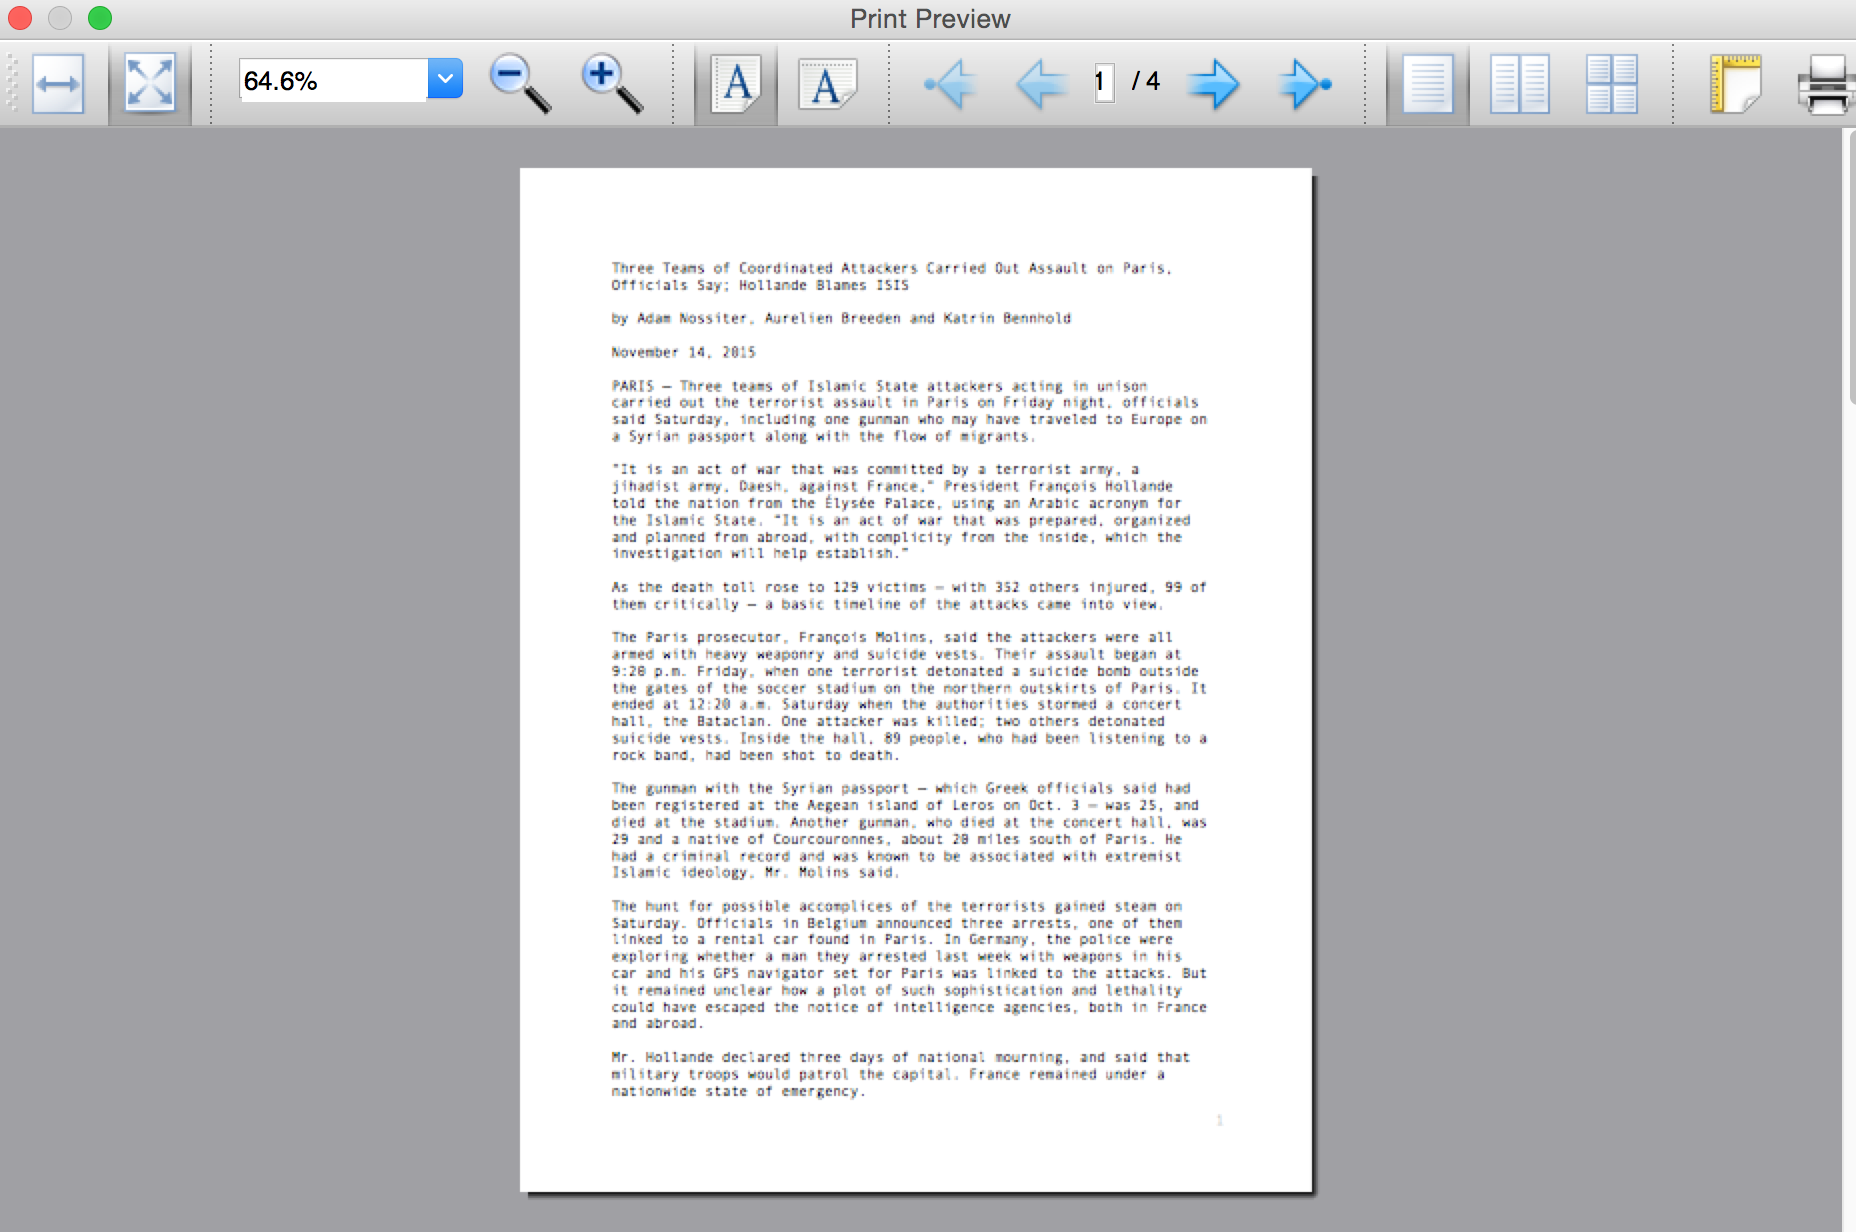
\includegraphics[width=\linewidth]{images/gui_screenshot_printpreview.png}
    \caption{The GUI screenshot of the print preview
      dialog.} \label{fig:gui_screenshot_printpreview}}
\end{figure}
Note, here I do not support or maintain this tool after I found out
about \href{https://www.readability.com}{Readability}.

\subsection{GUI2: Readability GUI Front-End} \label{subsec:gui2}
This is the PyQt4 GUI front-end to
\href{https://www.readability.com}{Readability}. A screenshot of the
list of articles widget is shown in
Fig.~(\ref{fig:gui2_screenshot_articlelist}, and a screenshot of the
article text widget is shown in
Fig.~(\ref{fig:gui2_screenshot_articletext}.
\begin{figure}[!ht]
  \parbox[!ht]{0.52\linewidth}{%
    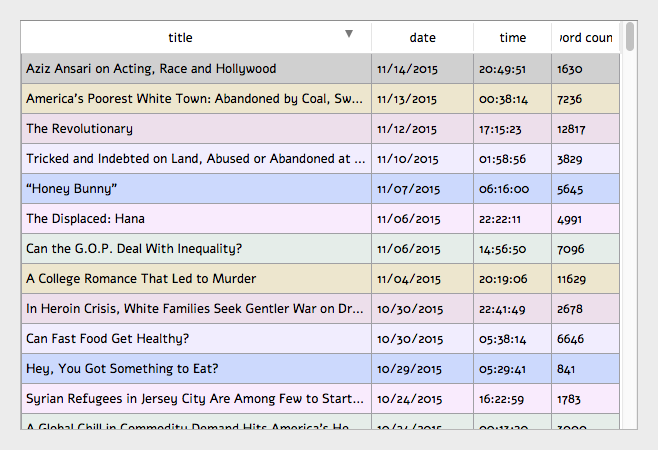
\includegraphics[width=\linewidth]{images/gui2_screenshot_articlelist.png}
    \caption{List of bookmarked (stored) articles under the user's
      account.} \label{fig:gui2_screenshot_articlelist} } \hfill
  \parbox[!ht]{0.45\linewidth}{%
    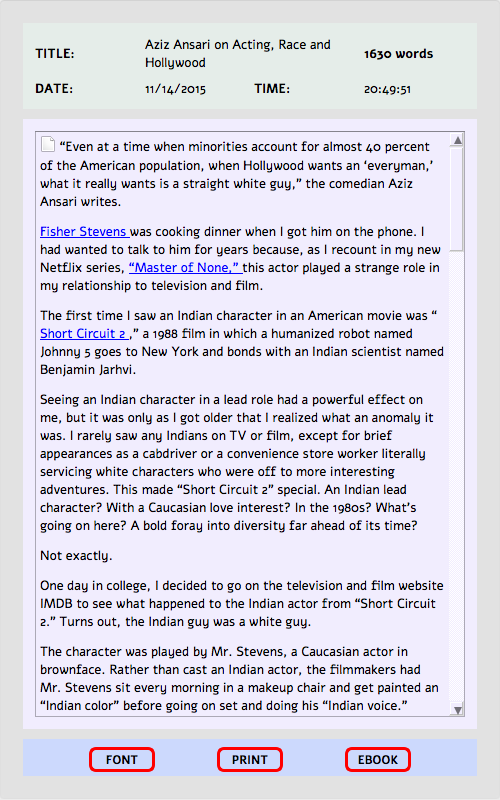
\includegraphics[width=\linewidth]{images/gui2_screenshot_articletext.png}
    \caption{The text form of the article's content, with working
      dialogs for \texttt{Font} and \texttt{Print
        Preview}.} \label{fig:gui2_screenshot_articletext} }
\end{figure}
A screenshot of the font changing dialog, the {\verb|Font|} button,
is shown in Fig.~(\ref{fig:gui2_screenshot_fontdialog}). A screenshot
of the print preview dialog, the {\verb|Print|} button, is shown in
Fig.~(\ref{fig:gui2_screenshot_printpreviewdialog}).
\begin{figure}[!ht]
  \parbox[!ht]{0.3\linewidth}{%
    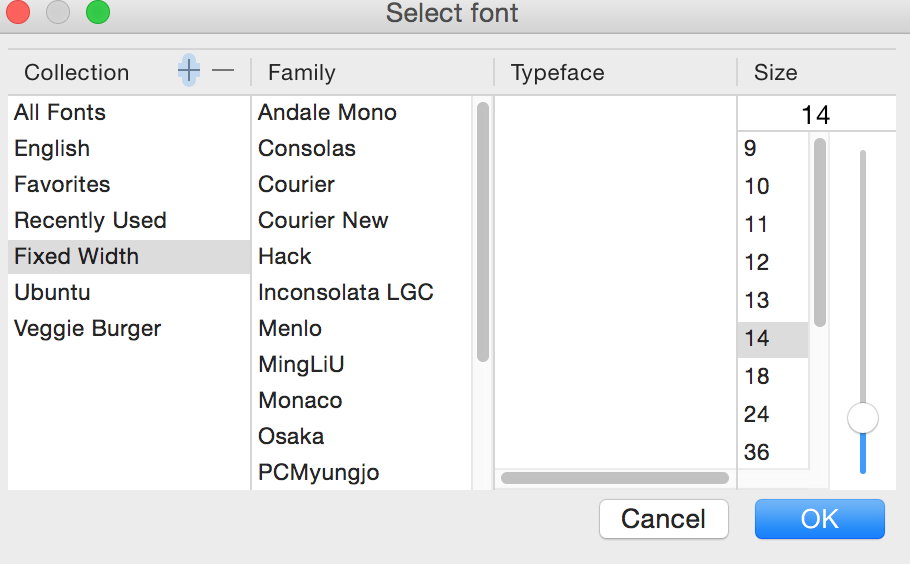
\includegraphics[width=\linewidth]{images/gui2_screenshot_fontdialog.png}
    \caption{The font changing dialog launched by the \texttt{Font}
      button in the article text widget. The initial preference for
      the font to display are fixed width
      fonts.} \label{fig:gui2_screenshot_fontdialog} } \hfill
  \parbox[!ht]{0.6\linewidth}{%
    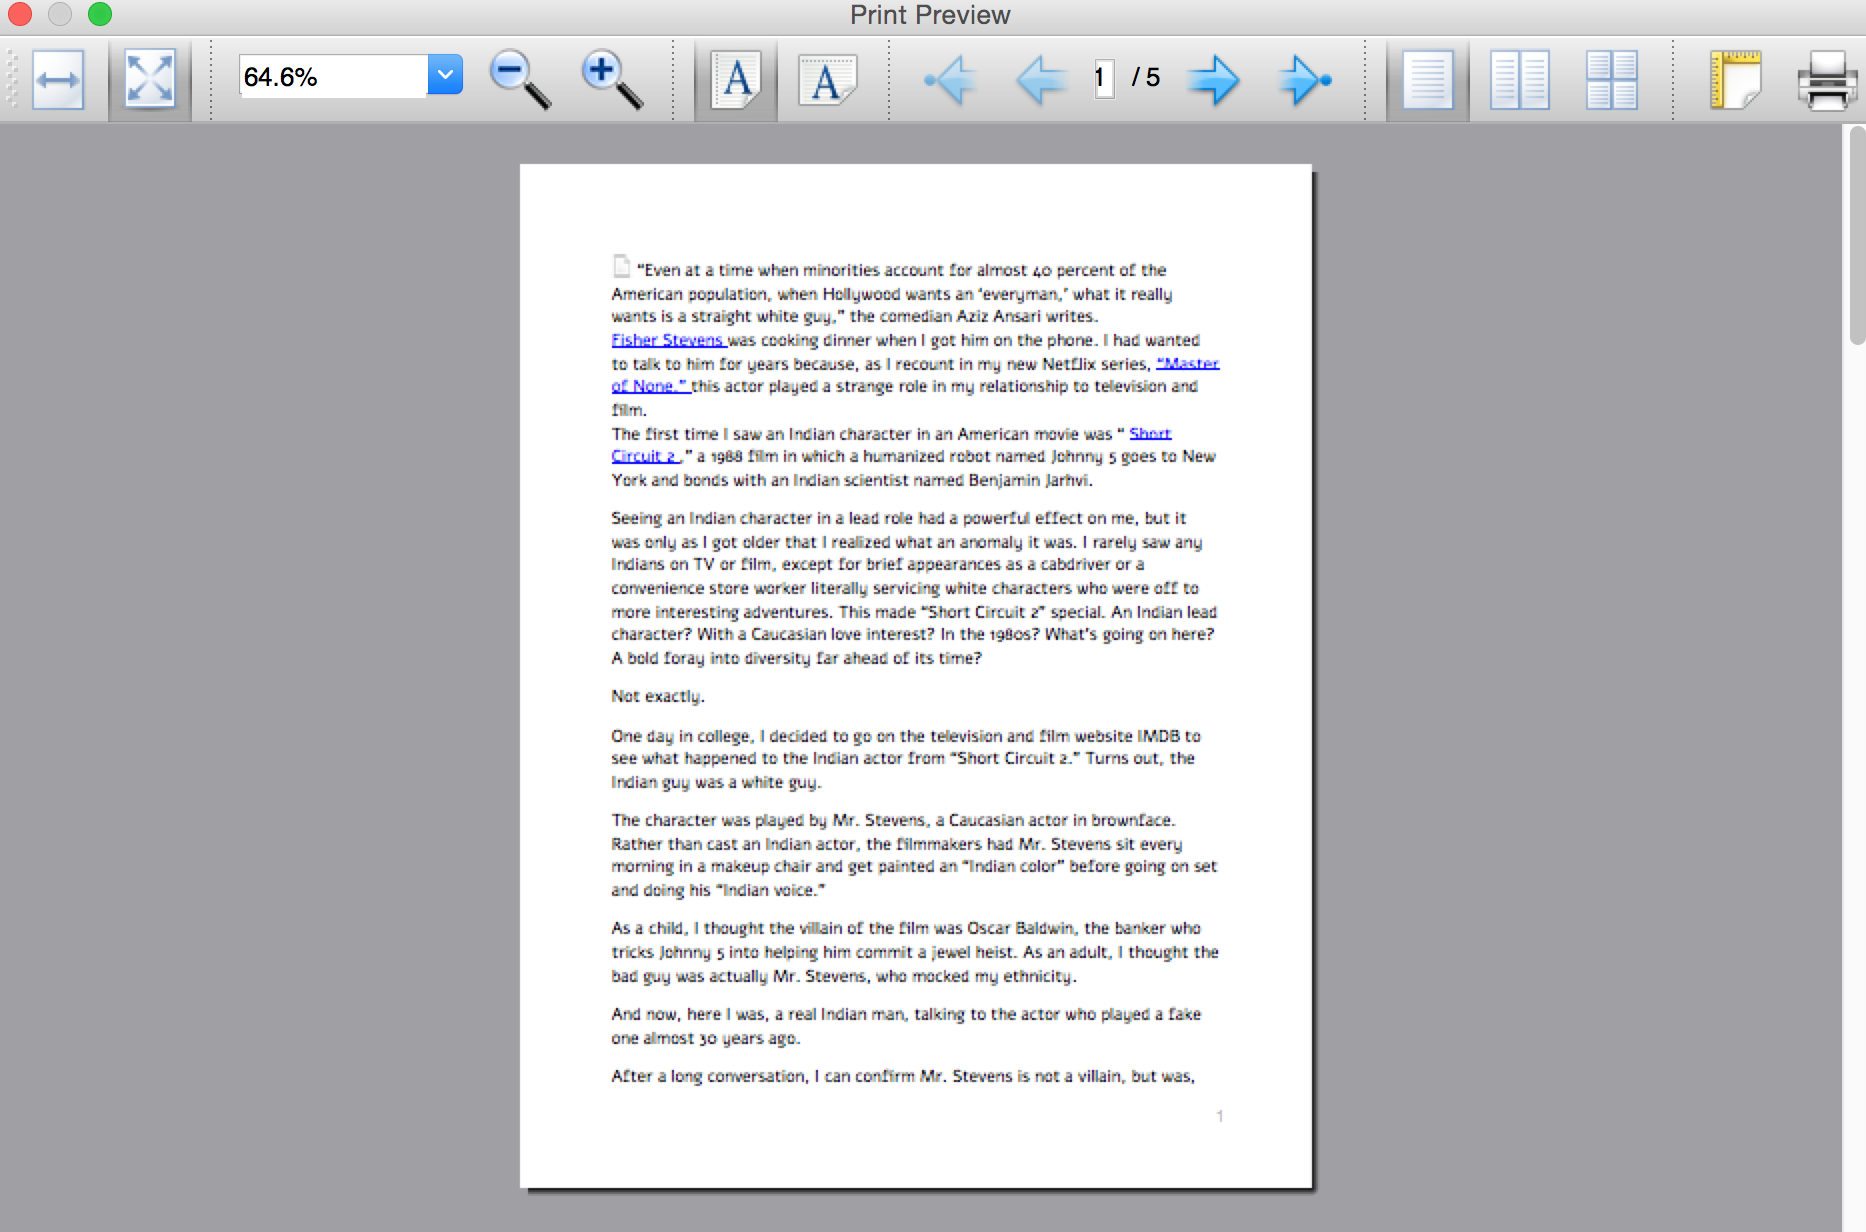
\includegraphics[width=\linewidth]{images/gui2_screenshot_printpreviewdialog.png}
    \caption{The print preview dialog launched by the \texttt{Print}
      button in the article text
      widget.} \label{fig:gui2_screenshot_printpreviewdialog} }
\end{figure}
In the immediate future, I plan on at least implementing the
follwoing, all using the Readability API.
\begin{itemize}
\item {\verb|EPUB|} button, to create the article in
  \href{https://en.wikipedia.org/wiki/EPUB}{EPUB} format.
  
\item Adding and deleting articles through the article list widget.
\end{itemize}

\section{Oldstuff}\label{sec:oldstuff}
These are tools that I do not maintain, located in the
{\verb|oldstuff|} folder, but which others may find
useful. These are pieces of code that I have started, but which are
unmaintained. These are the following pieces of code:
{\verb|freshair.sh|}, {\verb|waitwait.sh|}, and
{\verb|google_pull_contacts.py|}.

\end{document}
